% Structured DSS pass in 2D: nodal value propagating around a shared corner, three stages.
% Each contribution (a,b,c,d) is a distinct small marker; the corner circle accumulates
% markers as the dimensional passes merge neighbouring copies. The cells start fully
% separated, become adjacent along x after the x-pass, and fully merged after the y-pass.
\usetikzlibrary{arrows.meta, positioning, calc, shapes.geometric}
\scalebox{1.25}{%
    \begin{tikzpicture}[
        scale=0.95,
        every node/.style={font=\small},
        gridline/.style={gray!60, thin},
        ring/.style={draw=gray!75, thin, fill=white},
        exch/.style={{Stealth[length=2mm]}-{Stealth[length=2mm]}, thick, blue!60!black},
        mA/.style={circle, fill=red!80!black, inner sep=1.8pt},
        mB/.style={rectangle, fill=blue!70!black, inner sep=1.8pt},
        mC/.style={regular polygon, regular polygon sides=3, fill=green!55!black, inner sep=1.1pt},
        mD/.style={diamond, fill=orange!90!black, inner sep=1.4pt},
        ]

        % --- helpers -----------------------------------------------------------
        \def\mo{0.085} % marker offset inside a ring
        \newcommand{\setone}[2]{\node[#2] at #1 {};}
        \newcommand{\settwo}[3]{%
            \node[#2] at ($#1+(-\mo,0)$) {};
            \node[#3] at ($#1+(\mo,0)$) {};}
        \newcommand{\setfour}[1]{%
            \node[mA] at ($#1+(-\mo,\mo)$) {};
            \node[mB] at ($#1+(\mo,\mo)$) {};
            \node[mC] at ($#1+(-\mo,-\mo)$) {};
            \node[mD] at ($#1+(\mo,-\mo)$) {};}

        % text labels outside the rings, wide offset (multi-term sums)
        \newcommand{\lbls}[4]{%
            \node[font=\scriptsize] at ($(nw)+(-0.49,0.43)$) {$\substack{#1}$};
            \node[font=\scriptsize] at ($(ne)+(0.49,0.43)$)  {$\substack{#2}$};
            \node[font=\scriptsize] at ($(sw)+(-0.49,-0.43)$) {$\substack{#3}$};
            \node[font=\scriptsize] at ($(se)+(0.49,-0.43)$)  {$\substack{#4}$};}
        % text labels, close offset (single letters)
        \newcommand{\lblsc}[4]{%
            \node[font=\scriptsize] at ($(nw)+(-0.27,0.27)$) {$\substack{#1}$};
            \node[font=\scriptsize] at ($(ne)+(0.27,0.27)$)  {$\substack{#2}$};
            \node[font=\scriptsize] at ($(sw)+(-0.27,-0.27)$) {$\substack{#3}$};
            \node[font=\scriptsize] at ($(se)+(0.27,-0.27)$)  {$\substack{#4}$};}

        % four cells with x-gap #1 and y-gap #2; defines ring coords nw/ne/sw/se.
        % #3 = caption.
        \newcommand{\dsscells}[3]{%
            \pgfmathsetmacro\gx{#1/2}%
            \pgfmathsetmacro\gy{#2/2}%
            \begin{scope}[shift={(-\gx,\gy)}]   % NW
                \draw[gridline] (0,1.5) rectangle (1.5,3); \coordinate (nw) at (1.15,1.85);
                \node[ring, circle, minimum size=3.3mm] at (nw) {};
            \end{scope}
            \begin{scope}[shift={(\gx,\gy)}]    % NE
                \draw[gridline] (1.5,1.5) rectangle (3,3); \coordinate (ne) at (1.85,1.85);
                \node[ring, circle, minimum size=3.3mm] at (ne) {};
            \end{scope}
            \begin{scope}[shift={(-\gx,-\gy)}]  % SW
                \draw[gridline] (0,0) rectangle (1.5,1.5); \coordinate (sw) at (1.15,1.15);
                \node[ring, circle, minimum size=3.3mm] at (sw) {};
            \end{scope}
            \begin{scope}[shift={(\gx,-\gy)}]   % SE
                \draw[gridline] (1.5,0) rectangle (3,1.5); \coordinate (se) at (1.85,1.15);
                \node[ring, circle, minimum size=3.3mm] at (se) {};
            \end{scope}
            \node[align=center, font=\footnotesize] at (1.5,-0.7) {#3};}

        % ---- Stage 1: cells fully separated; one marker per ring; x-exchange arrows ----
        \begin{scope}[shift={(0,0)}]
            \dsscells{0.5}{0.5}{(a) initial}
            \setone{(nw)}{mA} \setone{(ne)}{mB} \setone{(sw)}{mC} \setone{(se)}{mD}
            \lblsc{a}{b}{c}{d}
            % x-pass sums every DoF along the shared vertical face, not just the corner
            \foreach \y in {2.1,2.55,3.0} \draw[exch] (1.1,\y) -- (1.9,\y);
            \foreach \y in {0.9,0.45,0.0} \draw[exch] (1.1,\y) -- (1.9,\y);
        \end{scope}

        \node at (3.95,1.5) {$\xrightarrow{\;x\text{-pass}\;}$};

        % ---- Stage 2: adjacent in x, separated in y; two markers per ring; y-exchange ----
        \begin{scope}[shift={(4.9,0)}]
            \dsscells{0}{0.5}{(b) after $x$-pass}
            \settwo{(nw)}{mA}{mB} \settwo{(ne)}{mA}{mB}
            \settwo{(sw)}{mC}{mD} \settwo{(se)}{mC}{mD}
            \lbls{a{+}b}{a{+}b}{c{+}d}{c{+}d}
            % y-pass sums every DoF along the shared horizontal face
            \foreach \x in {0.4,0.8,1.15} \draw[exch] (\x,1.9) -- (\x,1.1);
            \foreach \x in {1.85,2.2,2.6} \draw[exch] (\x,1.9) -- (\x,1.1);
        \end{scope}

        \node at (8.85,1.5) {$\xrightarrow{\;y\text{-pass}\;}$};

        % ---- Stage 3: fully merged; all four markers per ring; no arrows ----
        \begin{scope}[shift={(9.8,0)}]
            \dsscells{0}{0}{(c) after $y$-pass}
            \setfour{(nw)} \setfour{(ne)} \setfour{(sw)} \setfour{(se)}
            \lbls{a{+}b{+}\\c{+}d}{a{+}b{+}\\c{+}d}{a{+}b{+}\\c{+}d}{a{+}b{+}\\c{+}d}
        \end{scope}

    \end{tikzpicture}%
}
